% !TEX root = ../Thesis.tex
\chapter{Results}

In this chapter we will address the results gained so far. Looking first at the impact of laser illumination on coherence times before examining the impact of the Stark shift on selenium donors in purified silicon and the hyperfine coupling of phosphorus donors to $^{29}$Si nuclei in natural silicon.

\section{Illumination Induced Decoherence}

\subsection{Initial Measurements}

The first step undertaken before any laser illumination occurs is to characterise the sample's $T_1$ and $T_2$ times `in the dark' at the measurement temperature. 
Experiments were performed at 8k and 7k, with typical $T_1$ and $T_2$ decays shown in figure \ref{fig:t1andt2}.
The inversion recovery has be fitted with a standard exponential decay whilst the $T_2$ decay has had a stretched exponential decay applied.
The time constants of these decays give the $T_1$ and $T_2$ times with errors in the fit used to establish errors in their values.
The stretched exponential decay of $T_2$ indicates the presence of spectral diffusion.
$T_2$ decays with dynamical decoupling applied do not have this stretch factor as they are isolated from spectral diffusion.
At 8k $T_1$ was measured to be approximately $6.4\pm0.01$ms, with $T_2$ at approximately $240\pm2\mu$s.
At 7k $T_1$ was $32\pm0.1$ms and $T_2$ was unchanged.
A problem encountered in this work was some inconsistencies in $T_1$ at the same temperature but in different lab sessions.
The value at 8k was observed to vary between approximately 5ms and 7ms.
It is possible that this is attributable to different flow rates in the helium cryostat, meaning that use of a dry cryostat, which offers much greater temperature precision, would be beneficial. 


\begin{figure}
\centering
\begin{subfigure}[b]{0.5\textwidth}
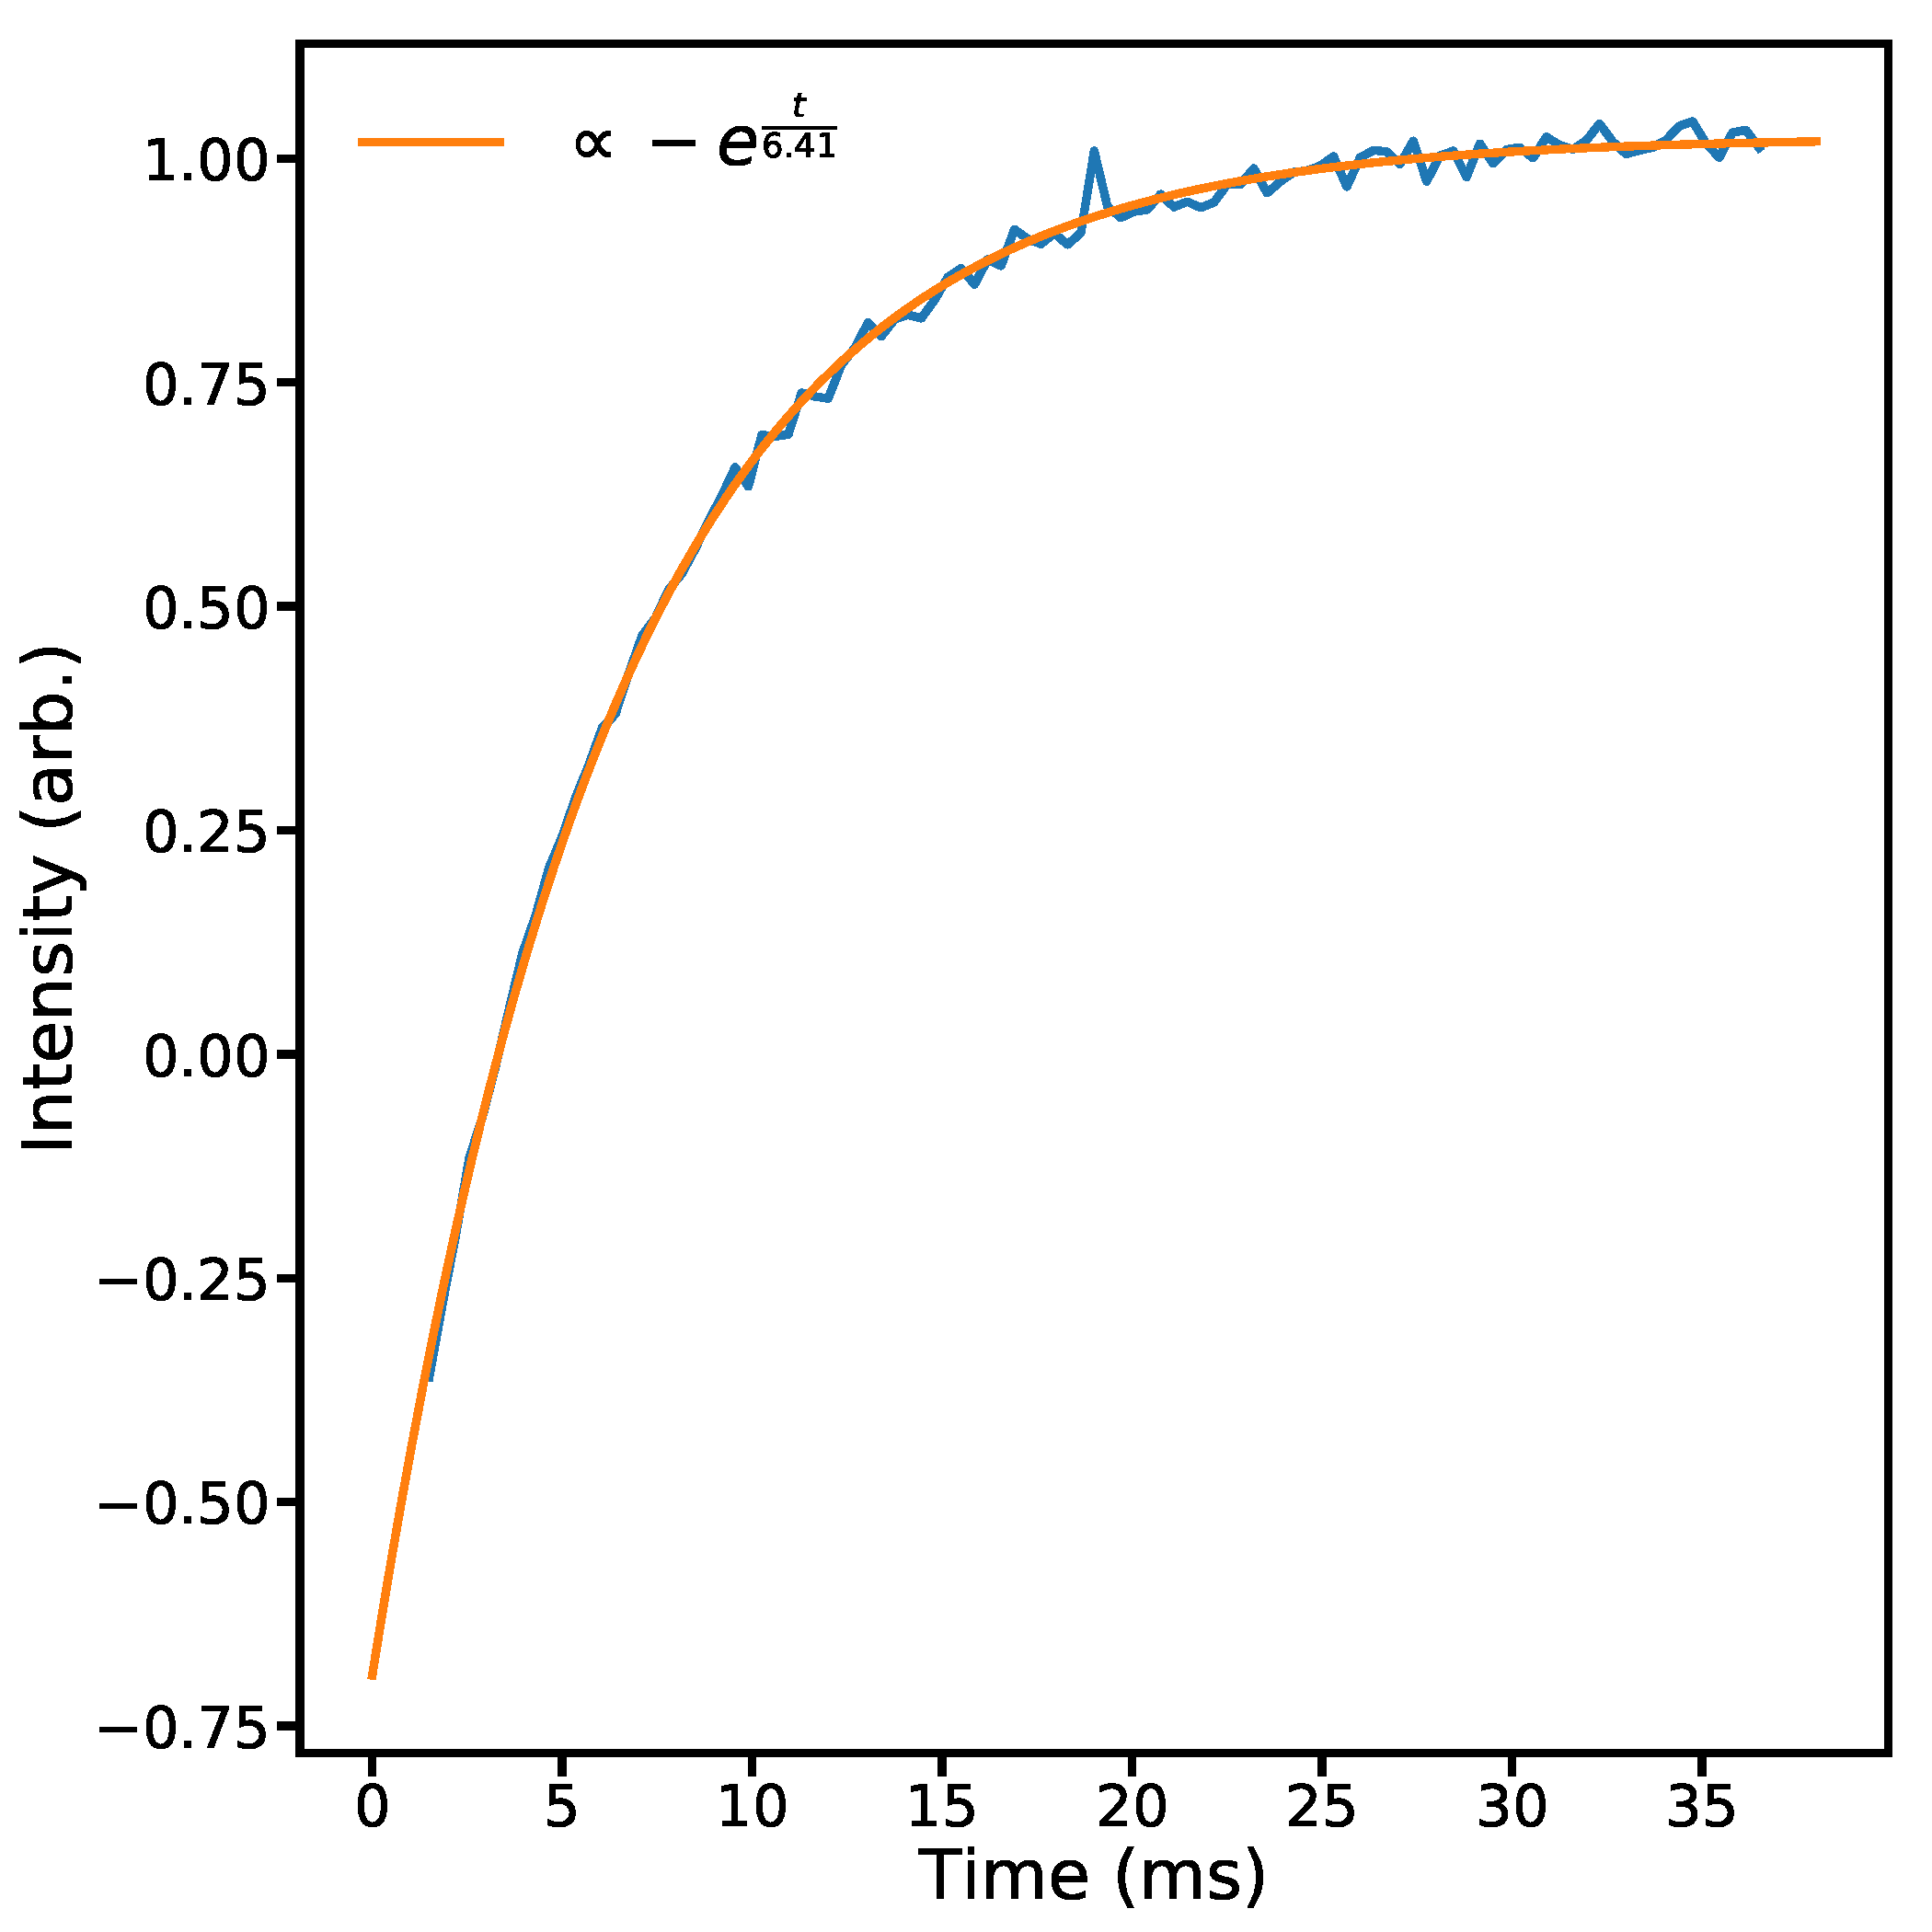
\includegraphics[width=\columnwidth]{Figures/T1Dark.pdf}{(a)}
\end{subfigure}%
\begin{subfigure}[b]{0.5\textwidth}
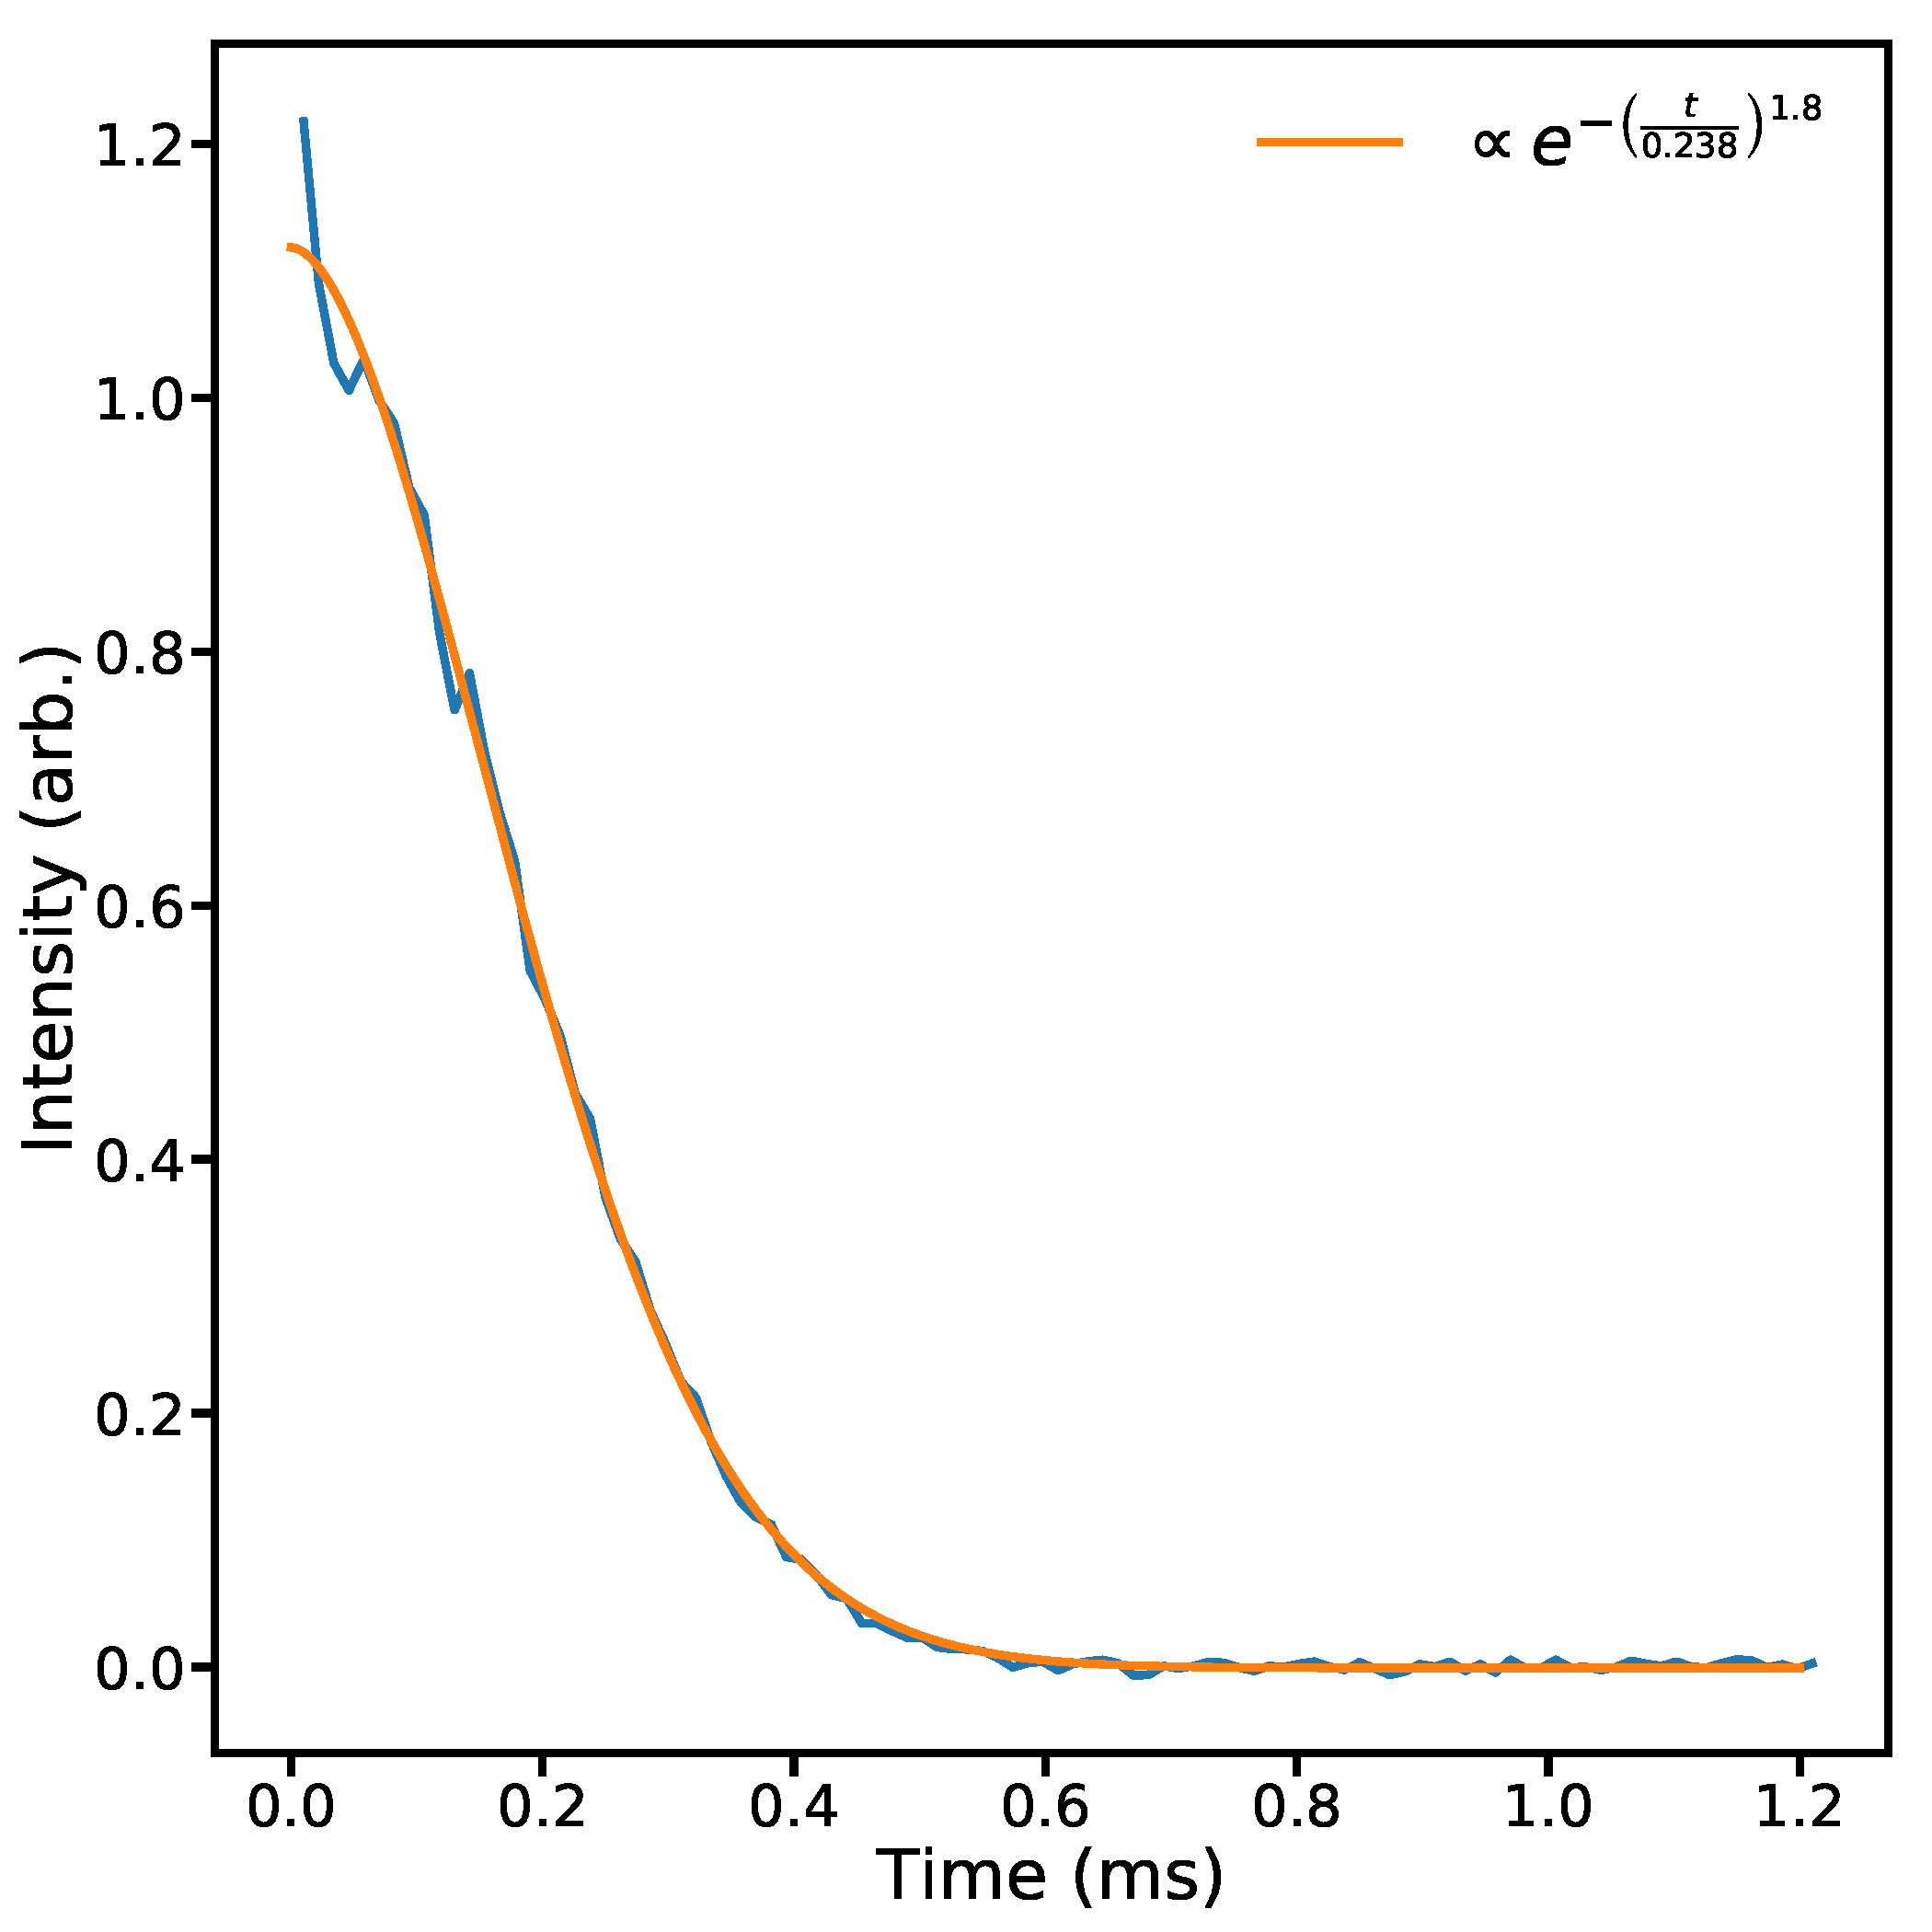
\includegraphics[width=\columnwidth]{Figures/T2Dark.pdf}{(b)}
\end{subfigure}%
\caption[$T_1$ and $T_2$ decays]{Typical $T_1$ and $T_2$ decays showing the inversion recovery for $T_1$ and the characteristic stretched exponential for $T_2$, indicating the presence of spectral diffusion.}
\label{fig:t1andt2}
\end{figure}

\subsection{High Power Measurements}

A set of high power measurements have been taken at powers between 2mW and 130mW, at wavelengths 1060nm, 1070nm and 1080nm, and at temperatures of 7k and 8k.
At each power and wavelength 3 measurements were made: $T_1$, $T_2$ and $T_2$ whilst using a 4 $\pi$ pulse dynamical decoupling sequence - CPMG.
An initial observation is that there is a strongly bi-exponential shape to the inversion recovery, requiring a fit of the form:

\begin{equation}
a e^{\frac{t}{T_{1a}}} + b e^{\frac{t}{T_{1b}}}
\end{equation}

this is clearly seen in figure \ref{fig:biexpDec}.

\begin{figure}
\centering
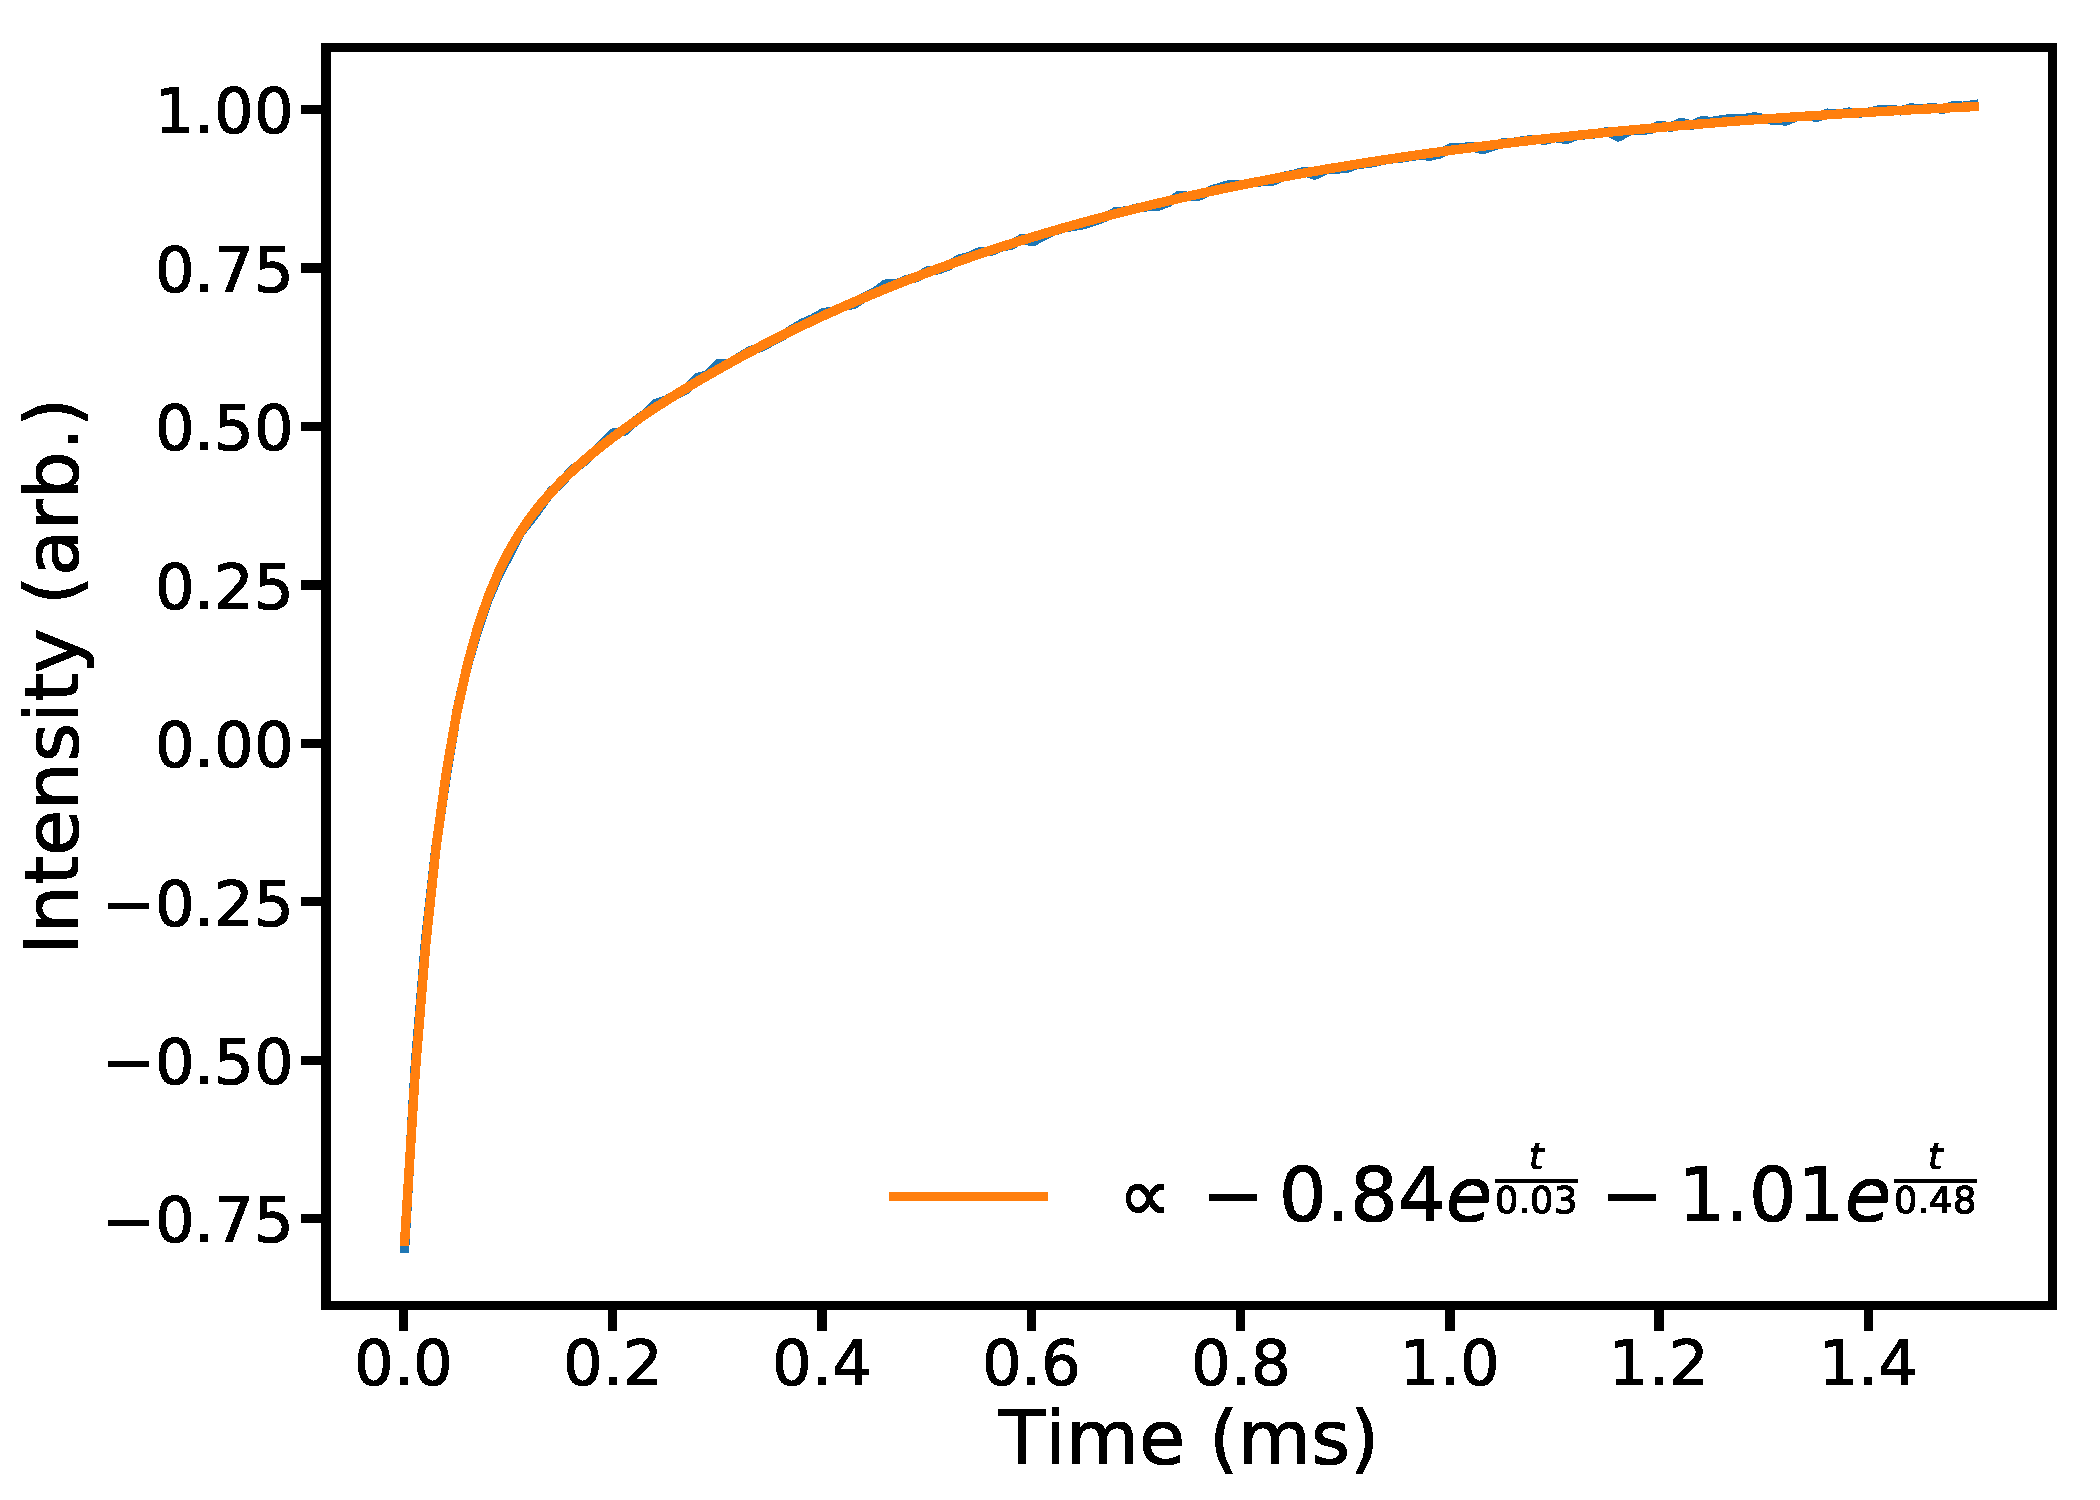
\includegraphics[width=0.8\textwidth]{Figures/T1_biExp.pdf}
\caption[Inversion recovery under laser illumination]{Inversion recovery at 8k and under 79mW illumination at 1070nm. Of note is the strongly bi-exponential nature of the decay, with two distinct time constants describing it. One significantly longer than the other. A possible explanation for this is that the laser illumination is not affecting all parts of the sample. This is not unexpected as the sample is quite large, as described in section \ref{sec:lasExps}}. 
\label{fig:biexpDec}
\end{figure}

Of the two time constants that describe the decay, one is significantly longer than the other and at low powers is close to the $T_1$ in the dark.
This suggests that there is a distribution of the illumination effect throughout the sample, with less affected parts relaxing more slowly than others 